\documentclass[10pt]{book}

%These tell TeX which packages to use.
\usepackage{array,epsfig}
\usepackage{amsmath}
\usepackage{amsfonts}
\usepackage{amssymb}
\usepackage{amsxtra}
\usepackage{amsthm}
\usepackage{mathrsfs}
\usepackage{color}
\usepackage{multicol}
\usepackage{enumitem}
%\usepackage{mdframed}
\usepackage[most]{tcolorbox}
\usepackage{pgfplots}
\usetikzlibrary{arrows}
\pgfplotsset{compat=1.6}

\pgfplotsset{soldot/.style={color=black,only marks,mark=*}} \pgfplotsset{holdot/.style={color=black,fill=white,only marks,mark=*}}

%Here I define some theorem styles and shortcut commands for symbols I use often
\theoremstyle{definition}
\newtheorem{defn}{Definition}
\newtheorem{thm}{Theorem}
\newtheorem{cor}{Corollary}
\newtheorem*{rmk}{Remark}
\newtheorem{lem}{Lemma}
\newtheorem*{joke}{Joke}
\newtheorem{ex}{Example}
\newtheorem*{soln}{Solution}
\newtheorem{prop}{Proposition}

\newcommand{\lra}{\longrightarrow}
\newcommand{\ra}{\rightarrow}
\newcommand{\surj}{\twoheadrightarrow}
\newcommand{\graph}{\mathrm{graph}}
\newcommand{\bb}[1]{\mathbb{#1}}
\newcommand{\Z}{\bb{Z}}
\newcommand{\Q}{\bb{Q}}
\newcommand{\R}{\bb{R}}
\newcommand{\C}{\bb{C}}
\newcommand{\N}{\bb{N}}
\newcommand{\M}{\mathbf{M}}
\newcommand{\m}{\mathbf{m}}
\newcommand{\MM}{\mathscr{M}}
\newcommand{\HH}{\mathscr{H}}
\newcommand{\Om}{\Omega}
\newcommand{\Ho}{\in\HH(\Om)}
\newcommand{\bd}{\partial}
\newcommand{\del}{\partial}
\newcommand{\bardel}{\overline\partial}
\newcommand{\textdf}[1]{\textbf{\textsf{#1}}\index{#1}}
\newcommand{\img}{\mathrm{img}}
\newcommand{\ip}[2]{\left\langle{#1},{#2}\right\rangle}
\newcommand{\inter}[1]{\mathrm{int}{#1}}
\newcommand{\exter}[1]{\mathrm{ext}{#1}}
\newcommand{\cl}[1]{\mathrm{cl}{#1}}
\newcommand{\ds}{\displaystyle}
\newcommand{\vol}{\mathrm{vol}}
\newcommand{\cnt}{\mathrm{ct}}
\newcommand{\osc}{\mathrm{osc}}
\newcommand{\LL}{\mathbf{L}}
\newcommand{\UU}{\mathbf{U}}
\newcommand{\support}{\mathrm{support}}
\newcommand{\AND}{\;\wedge\;}
\newcommand{\OR}{\;\vee\;}
\newcommand{\Oset}{\varnothing}
\newcommand{\st}{\ni}
\newcommand{\wh}{\widehat}
%Pagination stuff.
\setlength{\topmargin}{-0.75in}
\setlength{\oddsidemargin}{0in}
\setlength{\evensidemargin}{0in}
\setlength{\textheight}{9.in}
\setlength{\textwidth}{6.5in}
\pagestyle{empty}
\begin{document}
\begin{flushleft}
Name:\underline{\hspace{13cm}}Date:\underline{\hspace{2cm}}
\end{flushleft}
\begin{center}
{\Large Math 1041-012 \hspace{0.5cm} Section 5.4}
\end{center}
%\vspace{0.2 cm}

\begin{tcolorbox}
\subsection*{The Fundamental Theorem of Calculus (using antiderivatives)}
This is also called the \textit{Net Change} theorem.\\ \\
Suppose $f$ is \underline{\hspace{4cm}} on $[a,b]$, then
\[
\int_a^b f(x)\ dx = F(b)-F(a)
\]
where $F$ is the antiderivative of $f$, this means that \underline{\hspace{4cm}}.
\end{tcolorbox}
There are two basic types of problems:
\begin{itemize}
    \item {\huge$\displaystyle\int_a^b f(x)\ dx$} this is called a \underline{\hspace{4cm}} integral it will be a numerical answer!\vspace{1cm}
    \item {\huge$\displaystyle\int f(x)\ dx$} this is called an \underline{\hspace{4cm}} integral it will be the antiderivative\\  (don't for get $+C$).
\end{itemize}
Memorize the table of indefinite integrals below! You will be expected to know these.
\begin{figure}[h!]
    \centering
    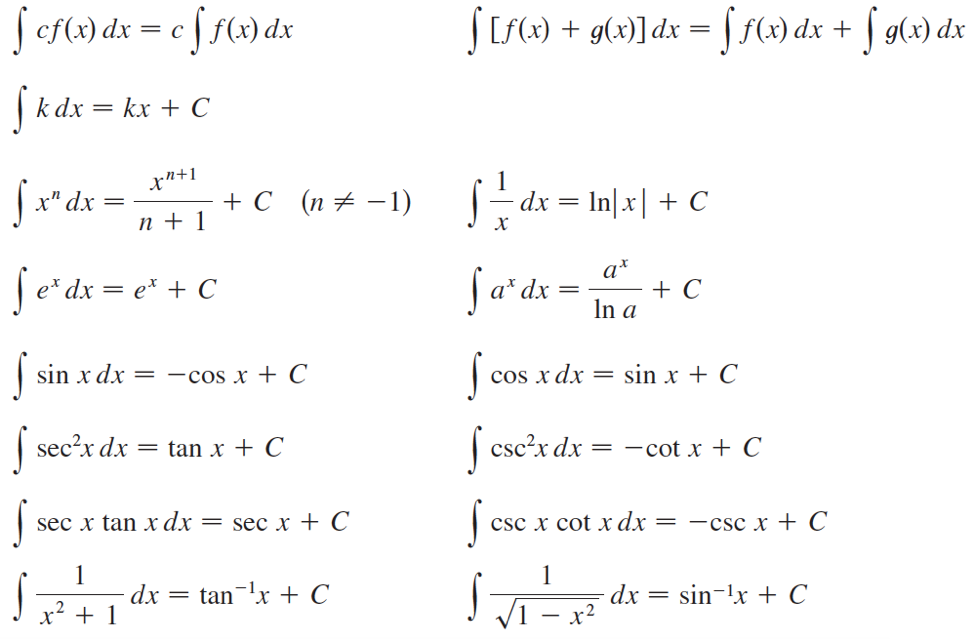
\includegraphics[width=5in]{basicIndefinites.png}
\end{figure}
\clearpage
\subsection*{Example 1: Finding Indefinite Integrals}
\begin{enumerate}[label=(\alph*)]
    \item Find the general antiderivative of $\displaystyle\int(10x^4-2\sec^2x)\ dx$\vspace{3cm}
    \item Evaluate $\displaystyle\int\frac{\cos\theta}{\sin^2\theta}\ d\theta$\vspace{3cm}
    \item $\displaystyle\int\frac{5}{x}+x^2(x+1)-4(1-x^2)^{-1/2}\ dx$\vspace{3cm}
\end{enumerate}
\subsection*{Example: Finding Definite Integrals}
\begin{enumerate}[label=(\alph*)]
    \item Evaluate $\displaystyle\int_0^3(x^3-6x)\ dx$\vspace{5cm}
    \clearpage
    \item Find $\displaystyle\int_0^2\left(2x^3-6x+\frac{3}{x^2+1}\right)\ dx$\vspace{5cm}
    \item Evaluate $\displaystyle\int_1^9\frac{2t^2+t^2\sqrt{t}-1}{t^2}\ dt$\vspace{6cm}
    \item Compute $\displaystyle\int_0^{\pi/4}\frac{1+\cos^2\theta}{\cos^2\theta}\ d\theta$
\end{enumerate}
\end{document}